% ---------------------------------------------------------------------------
% Paper B -- uncertainty-directed merit sortition under drift.
% ACM sigconf, anonymous review mode (same template as Paper A).
% Build:  tectonic main.tex
% Every number is regenerated by a script in ../code (paperB_complete.py, paperB_final.py,
% paperB_robust.py, paperB_attack.py); tables/*.tex are written by paperB_tables.py.
% ---------------------------------------------------------------------------
\documentclass[sigconf,anonymous,review,nonacm]{acmart}
\settopmatter{printacmref=false}
\renewcommand\footnotetextcopyrightpermission[1]{}
\pagestyle{plain}
\setcopyright{none}

\usepackage{booktabs}
\usepackage{amsmath}
\usepackage{xcolor}
\newcommand{\pending}[1]{\textcolor{red}{[#1]}}
\setlength{\emergencystretch}{2em}

\newtheorem{remark}{Remark}

\begin{document}

\title{Optimism Must Decay with Staleness: Uncertainty-Directed Merit Sortition Under Drift}

\author{Anonymous Author(s)}
\affiliation{\institution{Anonymous Institution}\country{}}

\begin{abstract}
Merit-based sortition chooses the active participants of a decentralized network by ranking
a smoothed record of their observed quality, and credits every unobserved participant with
the same imputed score. Treating each participant as an arm of a combinatorial bandit
replaces that shared imputation with per-participant uncertainty. We evaluate four such rules
against percentile sortition in four pool dynamics and three rates of latent-quality drift,
with every hyperparameter tuned on held-out seeds and every grid extended until no choice
sits on its boundary. Without drift, all four rules beat tuned percentile sortition in every
pool, by $6$--$17\%$ of its gain over random selection. Under drift the picture splits
by one property: whether a participant's uncertainty regrows while it goes unobserved. The
standard upper-confidence-bound rule, whose bonus depends on a lifetime observation count,
loses to tuned percentile sortition in $7$ of $8$ drift settings, by up to
$73\%$, even with a forgetting estimator. Discounted UCB, whose count decays, never
loses. Deployed with a single configuration and no knowledge of the drift rate, it is
never worse than, and in $4$ of $12$ settings better than, the best single percentile.
Infinite optimism for new identities invites whitewashing, and without a defence every
rule we test loses to percentile sortition under attack. A newcomer prior set at the
percentile that merit sortition already imputes makes Discounted UCB never worse than
percentile sortition at any attack strength, and better when a fifth of identities are
adversarial; its price is paid only where honest newcomers arrive often.
\end{abstract}

\keywords{sortition, decentralized systems, multi-armed bandits, non-stationarity, Sybil resistance, whitewashing}

\maketitle

% ===========================================================================
\section{Introduction}

Decentralized networks that pay for measurable work must decide, epoch after epoch, which
participants are \emph{active}. Merit-based sortition~\cite{kruijssen2024} ranks an
exponential moving average of each participant's observed quality and activates the top
$N_{\mathrm{act}}$. Inactive participants produce no observations, so every one of them is
credited with the same imputed value, the $P$-th percentile of the active set's
observations. The percentile $P$ is therefore a single, shared dose of optimism about
everyone who is not being watched. The Allora network uses it to choose an active set of
typically $32$ inferers~\cite{pfeffer2025context}.

A companion study~\cite{companionA} shows that adapting this scalar to the active set's
volatility does not help, and argues that the scalar is itself the bottleneck: the
information that should govern optimism is per participant, namely how much is known about
each one and how recently. Selecting the top $N_{\mathrm{act}}$ participants by an index
that combines an estimate with its uncertainty is exactly a combinatorial semi-bandit
policy~\cite{chen2013combinatorial,kveton2015tight}. This paper asks whether such policies
improve merit sortition, and what they need when participants' quality drifts.

\paragraph{The answer depends on one property.} We call a selection rule
\emph{staleness-aware} if a participant's uncertainty grows while it goes unobserved. The
standard upper-confidence-bound rule (UCB)~\cite{auer2002finite} is not: its exploration
bonus depends on a lifetime observation count, so a participant observed often, long ago,
looks well known no matter how stale its record is. Discounted UCB, sliding-window UCB
\cite{garivier2011switching}, and discounted Thompson sampling~\cite{raj2017taming} are.

\paragraph{Contributions.}
\begin{enumerate}
\item In a stationary pool, every uncertainty-directed rule we test beats percentile
sortition tuned to its best $P$, in all four pool dynamics of~\cite{kruijssen2024}, by
$6$--$17\%$ of percentile sortition's gain over random selection
(Section~\ref{sec:stationary}).
\item Under latent drift, UCB loses to tuned percentile sortition in $7$ of $8$
settings, by up to $73\%$ of that gain, even when its estimator forgets and its
exploration constant is tuned up to $c=2$. Forgetting in the estimate does not
substitute for staleness-aware uncertainty (Section~\ref{sec:drift}).
\item Discounted UCB never loses to tuned percentile sortition. Deployed with one
configuration chosen without knowledge of the pool or the drift rate, it is
never worse, and in $4$ of $12$ settings better, than the best single $P$
(Section~\ref{sec:deploy}).
\item Uncertainty-directed rules give new identities unbounded optimism, which a
whitewashing participant can exploit: undefended, every one of them loses to percentile
sortition under attack. A newcomer prior at the very percentile that merit sortition already
imputes makes D-UCB never worse than percentile sortition at any attack strength. It costs
nothing in a pool without honest arrivals and gives up D-UCB's stationary advantage in one
that has many (Section~\ref{sec:attack}).
\end{enumerate}
Every comparison is tuned and tested on disjoint seeds, scored on the unbiased metric
of~\cite{companionA}, extended past every grid boundary that a tuned choice touched, and
corrected for multiplicity. Section~\ref{sec:protocol} explains why each of these steps
changed a conclusion during this study.

% ===========================================================================
\section{Model and Selection Rules}
\label{sec:model}

\paragraph{Pool.} We use the simulation of~\cite{kruijssen2024} with its parameters. A pool
evolves over $1000$ epochs. At epoch $t$ the active set $A_t$, of size $N_{\mathrm{act}}$ or
the whole pool if smaller, is fielded, and each active participant $j$ produces an
observation $T_{tj}\sim\mathcal N(\tilde Q_{tj},V^2)$ with $V=0.2$. Latent qualities have
mean $\mu_Q=0.2$ and standard deviation $\sigma_Q=0.1$. The four pool dynamics (Fixed,
Growing, Shrinking, Evolving) differ in initial size, active-set size, Poisson growth and
geometric attrition, exactly as in~\cite{kruijssen2024,companionA}.

\paragraph{Drift.} To study non-stationarity we let latent quality follow a mean-reverting
Ornstein--Uhlenbeck process,
$\tilde Q_{t+1,j}=\tilde Q_{tj}+\theta(\mu_Q-\tilde Q_{tj})+\sigma_Q\sqrt{2\theta-\theta^2}\,\xi_{tj}$,
which holds the stationary standard deviation at $\sigma_Q$ for every $\theta$, so drift is
not confounded with a widening quality distribution. We test $\theta\in\{0,0.02,0.1\}$:
none, a half-life of about $35$ epochs, and about $7$ epochs.

\paragraph{Metric.} A run's score is the time average of $M_1$, the mean observation of the
fielded set before selection uses it. Scoring the newly selected set instead is biased
upward by an amount that grows with turnover, enough at these parameters to move tuned
optima~\cite{companionA}; it would favour exactly the high-exploration rules compared here.

\paragraph{Percentile sortition (static).} Each participant carries
$Q_{tj}=\alpha\hat Q_{tj}+(1-\alpha)Q_{t-1,j}$, $\alpha=0.1$, where $\hat Q_{tj}=T_{tj}$ if
$j$ is active and the $P$-th percentile of the active set's observations otherwise; the top
$N_{\mathrm{act}}$ by $Q$ are activated~\cite{kruijssen2024}. New arrivals start at the
current percentile.

\paragraph{Uncertainty-directed rules.} Each rule keeps, for each participant, an effective
count $N_j$ and a sum $S_j$ of its observations, activates the top $N_{\mathrm{act}}$ by an
index $I_j$, and sets $I_j=+\infty$ for a participant with no observation, so that every
newcomer is tried. Ties are broken at random.
\begin{itemize}
\item \textbf{UCB}~\cite{auer2002finite}: $N_j$ is the lifetime count, the estimate a running
mean with step $\max(1/N_j,\alpha_f)$, and $I_j=\bar T_j+c\sqrt{\log(t+1)/N_j}$. The floor
$\alpha_f\ge0$ lets the estimate forget; $\alpha_f=0$ is the plain sample mean.
\item \textbf{Discounted UCB (D-UCB)}~\cite{garivier2011switching}: every epoch,
$N_j\leftarrow\gamma N_j+\mathbf 1\{j\in A_t\}$ and $S_j\leftarrow\gamma S_j+T_{tj}\mathbf
1\{j\in A_t\}$, and $I_j=S_j/N_j+c\sqrt{\log(\sum_k N_k)/N_j}$.
\item \textbf{Sliding-window UCB (SW-UCB)}~\cite{garivier2011switching}: $N_j,S_j$ count the
last $\tau$ epochs only, and $I_j=S_j/N_j+c\sqrt{\log\min(t+1,\tau)/N_j}$, with
$I_j=+\infty$ if $j$ was not observed in the window.
\item \textbf{Discounted Thompson sampling (TS)}~\cite{agrawal2012thompson,raj2017taming}:
the statistics of D-UCB, and $I_j=S_j/N_j+s\,\zeta_j/\sqrt{N_j}$ with fresh
$\zeta_j\sim\mathcal N(0,1)$. With a flat prior and known noise, $s=V$ gives the posterior
sample; we tune $s$ like $c$.
\end{itemize}

\begin{remark}[Staleness]\label{rem:stale}
Let participant $j$ go unobserved for $u$ epochs. Under UCB its bonus changes only through
the slowly growing $\log(t+1)$; it does not depend on $u$. Under D-UCB its count is
multiplied by $\gamma^{u}$, so its bonus grows by the factor $\gamma^{-u/2}$, and the
participant is eventually re-examined however well it was once known. SW-UCB forgets
completely after $\tau$ epochs, and discounted TS widens its sampling distribution by the
same $\gamma^{-u/2}$. Percentile sortition sits in between: optimism is regranted to every
unobserved participant, but in one shared amount fixed by $P$.
\end{remark}

% ===========================================================================
\section{Protocol}
\label{sec:protocol}

\paragraph{Held-out tuning.} In every cell (pool $\times$ drift rate) each family's whole
grid is run on $50$ tuning seeds and the family's best configuration is picked there. The
picks are then re-run on $100$ disjoint evaluation seeds, shared across families so that
comparisons are paired. Picking and reporting on the same seeds inflates whichever family
has the larger grid~\cite{smith2006optimizer,cawley2010overfitting}.

\paragraph{No pick on a boundary.} A pick at the edge of its grid means the family's best
configuration may lie outside it. In a pilot, under strong drift, nearly every family's pick
sat on an edge, which would have favoured whichever family happened to have the widest
grid. We therefore widened every grid until no decisive pick touched a boundary
(Table~\ref{tab:grids}). Some limits are natural rather than truncations: $\alpha_f=0$,
$\gamma=1$ and $\tau=1000$ (the run length) mean no forgetting, $\alpha_f=1$ makes the
estimate the last observation, and $c=0$ for SW-UCB or $s=0$ for TS leaves no exploration
beyond trying every unobserved participant. In the final grid no pick, in any cell, lies on
any other boundary. At $\tau=1000$ SW-UCB never drops an observation and is the same rule as
UCB with $\alpha_f=0$; in the fixed pool without drift both families pick it, and their runs
are identical.

\paragraph{Inference.} Differences are paired, with $95\%$ intervals. ``Win'' and ``loss''
require a Holm-adjusted $p<0.05$ across all $108$ comparisons in the study;
``equivalent'' requires two one-sided tests~\cite{schuirmann1987tost,lakens2017equivalence}
to place the difference inside $\pm0.005$, which is $10\%$ of the merit-over-random
gap~\cite{companionA}. Gains are reported as a share of the gap between tuned percentile
sortition and random selection in the same cell.

\begin{table}[t]\centering\small
\caption{Tuning grids ($489$ configurations), identical in every cell.}
\label{tab:grids}
\setlength{\tabcolsep}{4pt}
\begin{tabular}{ll}
\toprule
Rule & Grid\\
\midrule
static & $P\in\{10,15,20,25,30,35,40,50,60,70,80\}\%$\\
UCB & $c\in[0.05,3]$ ($12$ values) $\times$ $\alpha_f\in[0,1]$ ($10$)\\
D-UCB & $c\in[0.01,0.6]$ ($9$) $\times$ $\gamma\in[0.6,1]$ ($12$)\\
SW-UCB & $c\in[0,0.6]$ ($11$) $\times$ $\tau\in\{3,\dots,1000\}$ ($10$)\\
TS & $s\in[0,0.4]$ ($10$) $\times$ $\gamma\in[0.5,1]$ ($14$)\\
\bottomrule
\end{tabular}
\end{table}

% ===========================================================================
\section{Without Drift, Every Rule Helps}
\label{sec:stationary}

\begin{table*}[t]\centering\small
\caption{Each rule against percentile sortition tuned to its best $P^\star$ (top) and rule
against rule (bottom), in every pool and drift rate: paired difference in $M_1$ on $100$
evaluation seeds, as a percentage of that cell's gap between tuned percentile sortition and
random selection. \textbf{Bold}: win, \underline{underlined}: loss (Holm-adjusted $p<0.05$
over all $108$ comparisons); otherwise equivalent within $\pm0.005$ by TOST.}
\label{tab:cells}
\setlength{\tabcolsep}{3.5pt}
\begin{tabular}{lrrrrrrrrrrrr}
\toprule
 & \multicolumn{4}{c}{$\theta=0$} & \multicolumn{4}{c}{$\theta=0.02$} & \multicolumn{4}{c}{$\theta=0.1$}\\
\cmidrule(lr){2-5}\cmidrule(lr){6-9}\cmidrule(lr){10-13}
Rule & Fix & Gro & Shr & Evo & Fix & Gro & Shr & Evo & Fix & Gro & Shr & Evo\\
\midrule
static $P^\star$ & 20\% & 25\% & 25\% & 30\% & 30\% & 35\% & 40\% & 35\% & 50\% & 50\% & 60\% & 50\%\\
\midrule
UCB & \textbf{+6.6} & \textbf{+14.0} & \textbf{+13.4} & \textbf{+14.0} & \underline{$-$9.4} & \underline{$-$43.4} & +2.9 & \underline{$-$12.0} & \underline{$-$12.4} & \underline{$-$72.6} & \underline{$-$11.5} & \underline{$-$26.9}\\
D-UCB & \textbf{+6.7} & \textbf{+16.6} & \textbf{+12.1} & \textbf{+10.8} & +0.6 & \textbf{+5.1} & $-$0.1 & +2.2 & +1.5 & +1.6 & +1.9 & +2.8\\
SW-UCB & \textbf{+6.6} & \textbf{+14.8} & \textbf{+13.3} & \textbf{+11.1} & $-$2.6 & +2.1 & $-$0.5 & +0.0 & \underline{$-$3.2} & \underline{$-$5.0} & $-$6.5 & $-$1.5\\
TS & \textbf{+6.3} & \textbf{+15.2} & \textbf{+12.9} & \textbf{+10.9} & $-$0.9 & +3.7 & +1.7 & +2.2 & $-$2.3 & +1.6 & $-$2.8 & +1.2\\
\midrule
UCB $-$ D-UCB & $-$0.1 & $-$2.7 & +1.3 & +3.1 & \underline{$-$10.0} & \underline{$-$48.5} & +3.0 & \underline{$-$14.2} & \underline{$-$13.8} & \underline{$-$74.2} & \underline{$-$13.4} & \underline{$-$29.8}\\
D-UCB $-$ SW-UCB & +0.1 & +1.8 & $-$1.2 & $-$0.2 & +3.2 & +3.0 & +0.4 & +2.2 & \textbf{+4.7} & \textbf{+6.6} & \textbf{+8.4} & \textbf{+4.3}\\
D-UCB $-$ TS & +0.4 & +1.5 & $-$0.8 & $-$0.0 & +1.5 & +1.3 & $-$1.8 & +0.0 & \textbf{+3.8} & +0.0 & +4.7 & +1.7\\
\bottomrule
\end{tabular}

\end{table*}

\begin{table*}[t]\centering\small
\caption{Configurations picked on the tuning seeds, per cell.}
\label{tab:picks}
\setlength{\tabcolsep}{4pt}
\begin{tabular}{llllll}
\toprule
$\theta$ & Pool & UCB & D-UCB & SW-UCB & TS\\
\midrule
$0$ & Fixed & $c{=}0.2,\,\alpha_f{=}0$ & $c{=}0.2,\,\gamma{=}1$ & $c{=}0.2,\,\tau{=}1000$ & $s{=}0.2,\,\gamma{=}1$\\
 & Growing & $c{=}0.15,\,\alpha_f{=}0$ & $c{=}0.1,\,\gamma{=}0.999$ & $c{=}0.2,\,\tau{=}1000$ & $s{=}0.1,\,\gamma{=}0.995$\\
 & Shrinking & $c{=}0.2,\,\alpha_f{=}0$ & $c{=}0.1,\,\gamma{=}0.999$ & $c{=}0.2,\,\tau{=}400$ & $s{=}0.1,\,\gamma{=}0.99$\\
 & Evolving & $c{=}0.15,\,\alpha_f{=}0$ & $c{=}0.03,\,\gamma{=}0.98$ & $c{=}0.3,\,\tau{=}800$ & $s{=}0.1,\,\gamma{=}0.995$\\
\midrule
$0.02$ & Fixed & $c{=}1.5,\,\alpha_f{=}0.02$ & $c{=}0.03,\,\gamma{=}0.85$ & $c{=}0.2,\,\tau{=}25$ & $s{=}0.02,\,\gamma{=}0.8$\\
 & Growing & $c{=}0.2,\,\alpha_f{=}0.1$ & $c{=}0.1,\,\gamma{=}0.95$ & $c{=}0.03,\,\tau{=}25$ & $s{=}0.03,\,\gamma{=}0.85$\\
 & Shrinking & $c{=}0.4,\,\alpha_f{=}0.02$ & $c{=}0.03,\,\gamma{=}0.85$ & $c{=}0.1,\,\tau{=}25$ & $s{=}0.05,\,\gamma{=}0.85$\\
 & Evolving & $c{=}0.4,\,\alpha_f{=}0.02$ & $c{=}0.02,\,\gamma{=}0.9$ & $c{=}0.1,\,\tau{=}25$ & $s{=}0.02,\,\gamma{=}0.85$\\
\midrule
$0.1$ & Fixed & $c{=}2,\,\alpha_f{=}0$ & $c{=}0.1,\,\gamma{=}0.85$ & $c{=}0.02,\,\tau{=}5$ & $s{=}0.05,\,\gamma{=}0.65$\\
 & Growing & $c{=}0.1,\,\alpha_f{=}0.3$ & $c{=}0.02,\,\gamma{=}0.75$ & $c{=}0.03,\,\tau{=}10$ & $s{=}0.03,\,\gamma{=}0.7$\\
 & Shrinking & $c{=}0.8,\,\alpha_f{=}0$ & $c{=}0.03,\,\gamma{=}0.75$ & $c{=}0.01,\,\tau{=}10$ & $s{=}0.05,\,\gamma{=}0.7$\\
 & Evolving & $c{=}0.8,\,\alpha_f{=}0$ & $c{=}0.02,\,\gamma{=}0.75$ & $c{=}0.1,\,\tau{=}10$ & $s{=}0.05,\,\gamma{=}0.75$\\
\bottomrule
\end{tabular}

\end{table*}

With fixed latent quality, all four uncertainty-directed rules beat percentile sortition at
its best $P$ in all four pools, by $6.3$--$16.6\%$ of percentile sortition's gain
over random selection (Table~\ref{tab:cells}). They are statistically equivalent to one
another in all $12$ pairwise comparisons with UCB. Without drift, every observation stays
informative, so whether uncertainty regrows is irrelevant, and the discounted rules choose
little or no discounting ($\gamma\ge0.98$, $\tau\ge400$; Table~\ref{tab:picks}).

% ===========================================================================
\section{Under Drift, Only Staleness-Aware Rules Survive}
\label{sec:drift}

Under drift, tuned percentile sortition becomes a much stronger baseline: its best $P$ rises
from $20$--$30\%$ without drift to $30$--$40\%$ at $\theta=0.02$ and
$50$--$60\%$ at $\theta=0.1$, regranting optimism to every unobserved participant
more generously. Against it, UCB loses in $7$ of $8$ drift settings, by
$9$--$73\%$ of the gap, and is equivalent in the remaining one (Table~\ref{tab:cells},
Figure~\ref{fig:rules}). Its
tuned configuration compensates with a very large exploration constant ($c$ up to $2$), which spreads
exploration evenly over everyone rather than towards whoever is stale.

Forgetting in the estimate does not repair it. The tuned forgetting floor $\alpha_f$ is
$0$--$0.3$, although the grid reaches $1$, and in three of the eight drift settings the best UCB uses no
forgetting at all. A stale estimate is harmless if the rule knows to revisit it, and
harmful if it does not; changing how fast the estimate moves does not change whether the
participant is revisited (Remark~\ref{rem:stale}).

\begin{figure*}[t]\centering
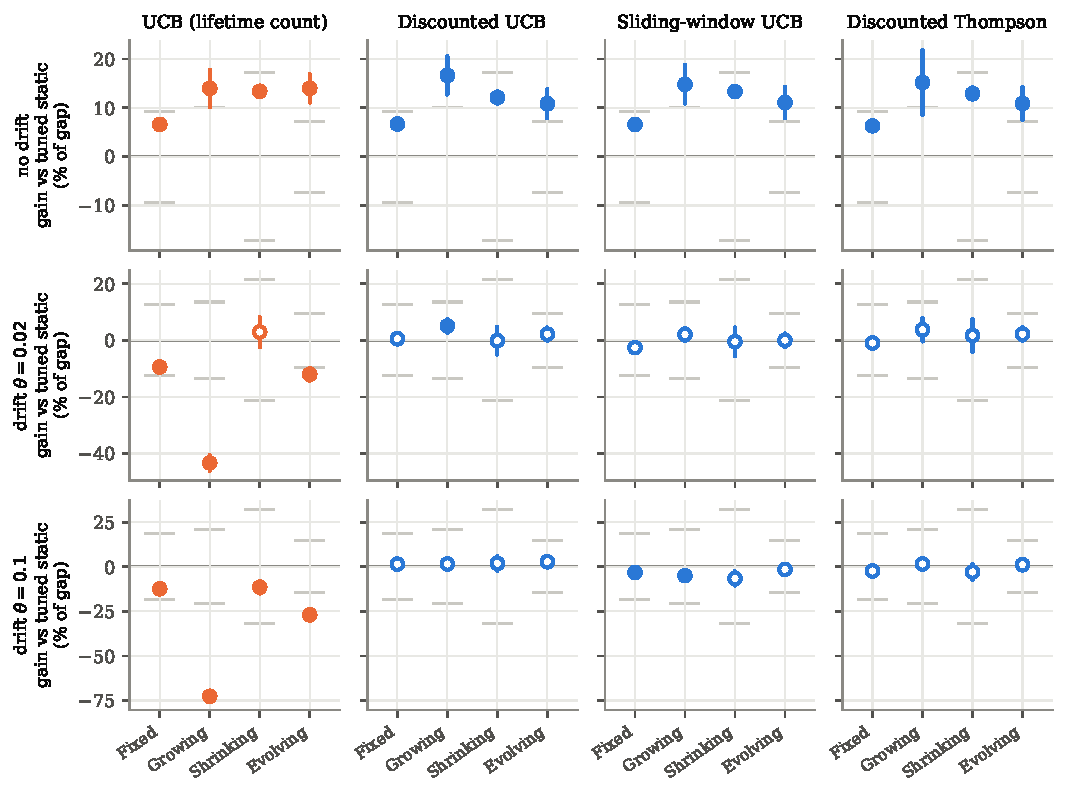
\includegraphics[width=0.92\textwidth]{figures/figB1_rule_vs_static.pdf}
\caption{Each uncertainty-directed rule against percentile sortition tuned to its best $P$,
as a percentage of that cell's gap between tuned percentile sortition and random selection
($100$ evaluation seeds, $95\%$ intervals). Rows: drift rate; columns: rule. Orange: an
exploration bonus from a lifetime count (UCB); blue: uncertainty that regrows while a
participant is unobserved. Filled markers are Holm-significant over all $108$ comparisons;
grey ticks mark the equivalence margin $\pm0.005$ in each pool's units.}
\label{fig:rules}
\end{figure*}

The three staleness-aware rules behave differently. D-UCB never loses to tuned percentile
sortition: it wins in $1$ drift setting and is equivalent in the other $7$. TS never loses
either. SW-UCB loses in two, both under strong drift, and at $\theta=0.1$ D-UCB beats it in
all four pools. The tuned configurations forget fast: $\gamma=0.75$--$0.95$ for D-UCB,
$\gamma=0.65$--$0.85$ for TS, and $\tau=5$--$25$ for SW-UCB. The grids had to reach that far.
Under strong drift TS's tuned discount is $0.65$--$0.75$ and D-UCB's $0.75$--$0.85$, below the
$0.95$ and $0.9$ at which our first grids stopped (Section~\ref{sec:protocol}).

Under drift, no rule clearly beats percentile sortition that is retuned for the drift rate:
D-UCB does so once.
What separates the rules is the cost of getting optimism wrong, which the next section
makes concrete.

% ===========================================================================
\section{Deploying Without Knowing the Drift}
\label{sec:deploy}

An operator must fix a configuration before knowing the pool's dynamics or its drift rate,
and percentile sortition's best $P$ moves from $20\%$ to $60\%$ across our settings. We
therefore score each family with a single configuration chosen by leave-one-cell-out: for
each held-out cell, the configuration with the lowest mean regret on the other $11$ cells.
Regret is the shortfall from the best configuration of any family in that cell, as a share
of that cell's gap. The held-out cell never influences the configuration it is scored with.

\begin{table}[t]\centering\small
\caption{One configuration per rule, chosen by leave-one-cell-out. Regret on the held-out
cell, as a percentage of its gap (mean and worst over the $12$ cells), and paired verdicts
against percentile sortition's leave-one-out choice on that cell's $50$ seeds, Holm-adjusted
across all cells and rules.}
\label{tab:deploy}
\setlength{\tabcolsep}{4pt}
\begin{tabular}{lrrcccc}
\toprule
Rule & mean & worst & win & loss & equiv. & inconcl.\\
\midrule
static & $13.5$ & $27.7$ & \multicolumn{4}{c}{(reference)}\\
UCB & $27.5$ & $79.2$ & 4 & 6 & 2 & 0\\
D-UCB & $12.0$ & $33.2$ & 4 & 0 & 8 & 0\\
SW-UCB & $23.1$ & $40.9$ & 0 & 7 & 5 & 0\\
TS & $16.8$ & $35.3$ & 2 & 1 & 8 & 1\\
\bottomrule
\end{tabular}

\end{table}

D-UCB is the only rule that is never worse than the best single percentile ($4$ wins,
$0$ losses, $8$ equivalent; Table~\ref{tab:deploy}), and it has the lowest mean regret
($12.0\%$ against $13.5\%$). Its worst-case regret is higher than percentile sortition's
($33.2\%$ against $27.7\%$, both in the growing pool without drift), but that cell's paired
comparison is equivalent. The choice is stable. Percentile sortition picks $P=40\%$ in all
$12$ folds, and D-UCB one of two neighbouring configurations ($c=0.03,\gamma=0.85$ or
$c=0.05,\gamma=0.9$, six folds each), so it is a stable recommendation rather than a lucky
one. TS loses once and is inconclusive once. SW-UCB loses in $7$ settings, including three
without drift, because its drift-agnostic window ($\tau=10$ or $25$) forgets too fast there.
UCB loses in $6$, all of them under drift.

% ===========================================================================
\section{Threat Model: Whitewashing}
\label{sec:attack}

Unbounded optimism for unobserved identities is a liability in an open network. If a new
identity is activated at once, a low-quality participant can abandon each identity as soon
as it is observed and deselected, and rejoin under a new one: whitewashing, a form of the
cheap-pseudonym and Sybil problems~\cite{friedman2001pseudonyms,douceur2002sybil,feldman2006freeriding}.
Percentile sortition is less exposed, because a newcomer starts at the $P$-th percentile
rather than above everyone.

\paragraph{Attack.} A fraction $a\in\{0,5,10,20\}\%$ of identities, in the initial pool and
among arrivals, is adversarial, with latent quality fixed at $\mu_Q-2\sigma_Q$. An
adversarial participant that has been observed and is not selected abandons its identity and
rejoins immediately as a fresh one, with the same quality and remaining lifetime. Rejoining is
free, the worst case for the defender. Each rule keeps the configuration it was tuned to on
honest pools (Table~\ref{tab:picks}): the defender does not tune against the attack. We run
the fixed and evolving pools at $\theta\in\{0,0.02\}$, $100$ paired seeds per arm, and
Holm-adjust the $144$ comparisons with percentile sortition in this experiment together.

\paragraph{Defence.} Give each newcomer, honest or not, a prior of $n_0$ pseudo-observations at
the $25$th percentile of the current active set's observations, the value percentile
sortition imputes at its recommended $P$~\cite{kruijssen2024}. A newcomer is then
ranked as a participant of median-like quality with modest uncertainty, not as an
unbounded unknown. Under D-UCB the prior decays like any observation, so a newcomer that is
never chosen regains optimism over time. We sweep $n_0\in\{1,3,10,30,100\}$ rather than
tune it, so that its price on an honest pool is visible.

\begin{table*}[t]\centering\small
\caption{Whitewashing. For each pool and drift rate: $M_1$ without attack ($a=0$) and with a
fifth of identities adversarial ($a=20\%$), and the adversaries' share of the active set at
$a=20\%$ (\%). Percentile sortition is given as $M_1$; every other rule as its paired
difference from percentile sortition in units of $10^{-3}$. \textbf{Bold}: win,
\underline{underlined}: loss (Holm-adjusted $p<0.05$ over $144$ comparisons). Rows marked
$+n_0$ add the newcomer prior to D-UCB's tuned configuration.}
\label{tab:attack}
\setlength{\tabcolsep}{3pt}
\begin{tabular}{lrrrrrrrrrrrr}
\toprule
 & \multicolumn{3}{c}{Fixed, $\theta=0$} & \multicolumn{3}{c}{Evolving, $\theta=0$} & \multicolumn{3}{c}{Fixed, $\theta=0.02$} & \multicolumn{3}{c}{Evolving, $\theta=0.02$}\\
\cmidrule(lr){2-4}\cmidrule(lr){5-7}\cmidrule(lr){8-10}\cmidrule(lr){11-13}
Rule & $a{=}0$ & $a{=}20\%$ & adv. & $a{=}0$ & $a{=}20\%$ & adv. & $a{=}0$ & $a{=}20\%$ & adv. & $a{=}0$ & $a{=}20\%$ & adv.\\
\midrule
static & 0.253 & 0.226 & 4.2 & 0.266 & 0.240 & 6.1 & 0.239 & 0.214 & 7.4 & 0.253 & 0.227 & 7.3\\
\midrule
UCB & \textbf{+3.6} & \underline{$-$34.5} & 27.7 & \textbf{+9.5} & \underline{$-$47.9} & 32.7 & \underline{$-$3.6} & \underline{$-$47.8} & 31.9 & \underline{$-$6.6} & \underline{$-$72.1} & 39.0\\
SW-UCB & \textbf{+3.6} & \underline{$-$34.5} & 27.7 & \textbf{+9.4} & \underline{$-$60.8} & 37.5 & $-$0.5 & \underline{$-$30.2} & 23.9 & +0.1 & \underline{$-$41.6} & 27.1\\
TS & \textbf{+3.4} & \underline{$-$20.2} & 19.3 & \textbf{+9.6} & \underline{$-$32.6} & 24.8 & +0.5 & \underline{$-$23.0} & 20.4 & \textbf{+2.0} & \underline{$-$37.3} & 25.6\\
D-UCB & \textbf{+3.6} & \underline{$-$36.6} & 28.8 & \textbf{+8.5} & \underline{$-$36.1} & 26.5 & +0.7 & \underline{$-$22.0} & 20.3 & +1.2 & \underline{$-$37.3} & 25.7\\
\quad $+\,n_0{=}1$ & \textbf{+3.6} & \underline{$-$35.9} & 28.5 & \textbf{+7.7} & \textbf{+8.1} & 4.7 & +0.7 & \underline{$-$4.4} & 10.5 & +0.4 & \textbf{+4.9} & 5.7\\
\quad $+\,n_0{=}3$ & \textbf{+3.6} & \underline{$-$33.9} & 27.4 & \textbf{+6.3} & \textbf{+11.1} & 2.4 & +0.7 & +0.4 & 7.2 & +0.7 & \textbf{+7.6} & 3.8\\
\quad $+\,n_0{=}10$ & \textbf{+3.6} & \underline{$-$7.0} & 11.5 & \textbf{+3.2} & \textbf{+9.8} & 1.6 & +0.7 & \textbf{+3.8} & 5.2 & $-$0.5 & \textbf{+9.0} & 2.8\\
\quad $+\,n_0{=}30$ & \textbf{+3.6} & \textbf{+6.3} & 1.6 & $-$0.4 & \textbf{+7.9} & 1.5 & +0.7 & \textbf{+6.1} & 4.3 & $-$0.6 & \textbf{+10.3} & 2.6\\
\quad $+\,n_0{=}100$ & \textbf{+3.6} & \textbf{+8.0} & 0.2 & $-$2.8 & \textbf{+4.2} & 1.8 & +0.7 & \textbf{+6.2} & 3.7 & $-$1.0 & \textbf{+8.4} & 2.6\\
\bottomrule
\end{tabular}

\end{table*}

\begin{figure*}[t]\centering
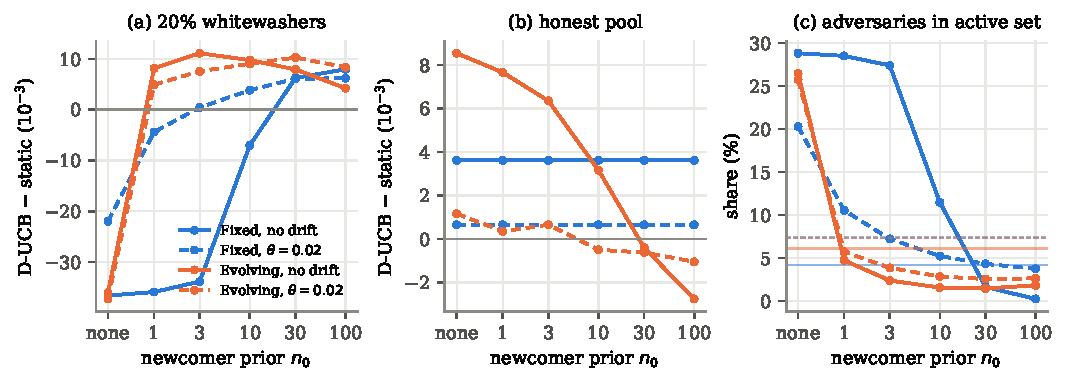
\includegraphics[width=\textwidth]{figures/figB2_whitewashing.pdf}
\caption{The newcomer prior as a defence, as its strength $n_0$ grows (``none'' is
undefended D-UCB). (a) With a fifth of identities whitewashing and (b) on an honest pool:
D-UCB's paired difference from percentile sortition, in units of $10^{-3}$ ($100$ seeds).
(c) Adversaries' share of the active set under attack; thin horizontal lines give
percentile sortition's share in the same cell.}
\label{fig:ww}
\end{figure*}

\paragraph{Results.} Undefended, the attack works against every uncertainty-directed rule
(Table~\ref{tab:attack}). With a fifth of identities adversarial, adversaries hold
$19$--$39\%$ of the active set under the four bandit rules, against $4$--$7\%$ under
percentile sortition, and every bandit rule loses to it in all four settings. The prior
closes the exposure progressively. At $n_0=30$ adversaries hold at most $4.3\%$, and D-UCB is
never worse than percentile sortition at any attack strength in any setting
(Figure~\ref{fig:ww}; the
$a=5\%$ and $10\%$ levels, not shown, are wins or equivalences too), and better at $a=20\%$
in all four.

The prior needed depends on the pool. D-UCB's bonus is $c\sqrt{\log(\sum_k N_k)/N_j}$, and in
a long-lived pool with little discounting the total count is large, about $5\times10^4$ in the
fixed pool without drift. A few pseudo-observations then still leave a newcomer far above the
incumbents: there $n_0=3$ cuts the adversaries' share only from $28.8\%$ to $27.4\%$, while
in the evolving pool it already wins under attack. Its price is paid only by honest newcomers.
The fixed pool has none, so no $n_0$ costs anything there. In the evolving pool without drift,
$n_0=30$ takes D-UCB's honest advantage over percentile sortition from $+8.5\times10^{-3}$ to
equivalence, and smaller priors keep more of it but defend less.

% ===========================================================================
\section{Related Work}

\emph{Sortition and committee selection.} Random selection with fairness
guarantees~\cite{flanigan2021fair} and cryptographic sortition~\cite{gilad2017algorand}
select without regard to measured performance; merit-based sortition~\cite{kruijssen2024}
weights selection towards it while keeping a path back for everyone. Reputation systems such
as EigenTrust~\cite{kamvar2003eigentrust} aggregate trust but do not decide whom to observe
next.

\emph{Bandits.} Top-$k$ selection on noisy rewards is a combinatorial
semi-bandit~\cite{chen2013combinatorial,kveton2015tight}. Non-stationary bandits use
discounting or windows~\cite{garivier2011switching}, with matching lower bounds that
depend on the variation budget~\cite{besbes2014nonstationary}; discounted Thompson sampling
adapts the same idea to posterior sampling~\cite{raj2017taming}. Our contribution is not a
new bandit algorithm but the finding that, in merit sortition, the property that separates
rules which help from rules which hurt is staleness-awareness, and that a held-out,
boundary-checked evaluation is needed to see it.

\emph{Identity attacks.} Cheap pseudonyms make reputation resettable
\cite{friedman2001pseudonyms}, and whitewashing exploits generous treatment of newcomers in
peer-to-peer systems~\cite{feldman2006freeriding}. Optimism in the face of uncertainty is a
particularly generous treatment; it can also be exploited by manipulating the rewards a UCB
learner observes~\cite{kocabay2026optimism}, whereas whitewashing needs only fresh
identities.

% ===========================================================================
\section{Discussion and Limitations}

\paragraph{What the percentile was doing.} Percentile sortition's $P$ is a crude form of
staleness-aware optimism: everyone unobserved is regranted the same score every epoch.
Under strong drift that crude form, retuned, is as good as anything we tested, which is why
retuned static is hard to beat. Its weakness is that the right $P$ depends on the drift rate,
which an operator does not know. D-UCB makes optimism per participant and proportional to
staleness, and one configuration then works across conditions. The newcomer prior completes
the correspondence: the percentile survives as the prior, not as the score.

\paragraph{Limitations.} All results are simulations in the model of~\cite{kruijssen2024},
with Gaussian noise and Ornstein--Uhlenbeck drift. Grids are finite even after extension.
The prior strength $n_0$ is swept, not tuned, and the value that suffices depends on how
long-lived the pool is. The attack is one strategy, worst case in its cost to the attacker
but not adaptive to the defence; collusion and strategic misreporting are out of scope. The equivalence margin is a
judgement; all intervals are reported.

\paragraph{A methodological note.} Before this protocol, an analysis that fixed $P$ and $c$
across drift rates and picked the forgetting rate on the seeds it reported concluded that UCB
with forgetting beats percentile sortition under drift. Tuning each family on held-out seeds
for each drift rate reversed that conclusion. The companion paper~\cite{companionA} documents
a related failure; together they argue that a mechanism's evaluation deserves as much care as
its design.

\section{Conclusion}
Uncertainty-directed selection improves merit sortition when the pool is stationary, and
under drift it helps only if a participant's uncertainty regrows while it is unobserved.
Discounted UCB has that property, never loses to tuned percentile sortition, and needs no
knowledge of the drift rate. Undefended, its optimism about new identities is exploitable;
with a newcomer prior at the percentile it resists whitewashing, at a price paid only where
honest newcomers are frequent.

\bibliographystyle{ACM-Reference-Format}
\bibliography{refs}

\end{document}
